\documentclass{beamer}
% \usepackage{lmodern}
%=====================================================================
% Color definition
\definecolor{jvagreen}{RGB}{0,104,	139}
\definecolor{jvagold}{RGB}{255, 255, 255}
\setbeamercolor{section in head/foot}{fg = jvagold, bg = jvagreen}
\usepackage{graphicx}
\usepackage{mathtools}
\usepackage{picture}
\usepackage{amsmath}
\usepackage{multimedia}
\DeclareMathOperator{\Tr}{Tr}
%\graphicspath{{../}}
\setbeameroption{show notes}
\usepackage{multicol}
\usepackage{caption}
\usepackage{textpos}

\usebackgroundtemplate
{
    
\includegraphics[width=\paperwidth,height=\paperheight]{img/blank.jpg}%
}
\beamertemplatenavigationsymbolsempty

%=====================================================================
% Templates - headline, frametitle

\makeatletter
% Komprimiert die miniframe Kreise auf eine Linie
\beamer@compresstrue
\makeatother

% Definiert die headline
\setbeamertemplate{headline}
{ 
%\includegraphics[width=\paperwidth]{pic} % test logo
\begin{beamercolorbox}[wd=\paperwidth,right]{section in head/foot}
    \rule{\paperwidth}{1pt}
    %Vertikaler Abstand
    \vskip20pt
    %Fügt die Standard-Navi ein (miniframes)
    %\insertnavigation{\paperwidth}
    \vskip8pt
    %\rule{\paperwidth}{0.5pt}
    %\vskip25.5pt % same height of the example provided, but IMHO is too much
    \rule{\paperwidth}{1pt}
\end{beamercolorbox} 
}
\setbeamertemplate{footline}
{ 
%\includegraphics[width=\paperwidth]{pic} % test logo
\begin{beamercolorbox}[wd=\paperwidth,right]{section in head/foot}
    \rule{\paperwidth}{1pt}
    %Vertikaler Abstand
    \vskip10pt
    %Fügt die Standard-Navi ein (miniframes)
    \insertnavigation{\paperwidth}
    \vskip8pt
    \rule{\paperwidth}{0.5pt}
    %\vskip25.5pt % same height of the example provided, but IMHO is too much
    %\rule{\paperwidth}{1pt}
\end{beamercolorbox} 
}

% definition of the frametitle
\setbeamertemplate{frametitle}
{
\vskip-24pt % to shift up the frametitle
\hbox{ 
 \begin{beamercolorbox}[wd=.0675\textwidth]{} % left shift
 \end{beamercolorbox} 
 \begin{beamercolorbox}[sep=4pt]{section in head/foot}
 \insertframetitle
 \end{beamercolorbox} 
 }
}

\mode<presentation>
{
    \setbeamertemplate{itemize item}[circle]
    \setbeamercolor{itemize item}{fg = jvagreen}
    \setbeamertemplate{itemize subitem}[circle]
    \setbeamercolor{itemize subitem}{fg = jvagreen}
}

\renewcommand\footnoterule{}

\AtBeginSection[]
{
  \begin{frame}<beamer>
    \frametitle{Outline}
    \tableofcontents[currentsection]
  \end{frame}
}

%\logo{\includegraphics[height=0.6cm]{img/cde_basic_green}}
%\let\oldequation=\equation
%\let\endoldequation=\endequation
%\renewenvironment{equation}{\vspace{1cm}\begin{oldequation}}{\end{oldequation}\vspace{15mm}}

\begin{document}

\addtobeamertemplate{frametitle}{}{%
\begin{textblock*}{100mm}(-0.9cm,-0.6cm)

\includegraphics[height=0.5cm,width=1.5cm]{img/uob-logo-white-transparent}
\end{textblock*}
\begin{textblock*}{100mm}(0.97\textwidth,-0.6cm)

\includegraphics[height=0.5cm,width=1cm]{img/cde_tag_white}
\end{textblock*}
}

\title[Performance-driven Facial Animation]{
  Performance-driven Facial Animation}

% Optional: a subtitle to be dispalyed on the title slide
% \subtitle{Show where you're from}
% \subtitle{Presented by: Ieva Kazlauskaite}
% The author(s) of the presentation:
%  - again first a short version to be displayed at the bottom;
%  - next the full list of authors, which may include contact information;
\author[Garoe Dorta Perez, Ieva Kazlauskaite, Richard Shaw]{
   Garoe Dorta Perez, Ieva Kazlauskaite, Richard Shaw } 


% The institute:
%  - to start the name of the university as displayed on the top of each slide
%    this can be adjusted such that you can also create a Dutch version
%  - next the institute information as displayed on the title slide
\institute[University of Bath]{
University of Bath \\
Centre For Digital Entertainment
}

% Add a date and possibly the name of the event to the slides
%  - again first a short version to be shown at the bottom of each slide
%  - second the full date and event name for the title slide

\date{27 May 2015}

% TITLE PAGE
\begin{frame}[plain]
  \titlepage
\end{frame}

%\section{Overview}
% CONTENT PAGE
%\begin{frame}
%  \frametitle{Overview}
%  \tableofcontents
%\end{frame}

%----------------------------------------------------------------------
\section{Richard's Part}
\begin{frame}{Data Capture}

\begin{itemize}
\setlength\itemsep{0.5em}
\item Performance capture using two DSLR cameras in stereo.
\item Video recorded at 60fps with resolution $640 \times 480$ pixels.
\item Video streams synchronised using audio signals.
\end{itemize}

\begin{center}
\begin{figure}
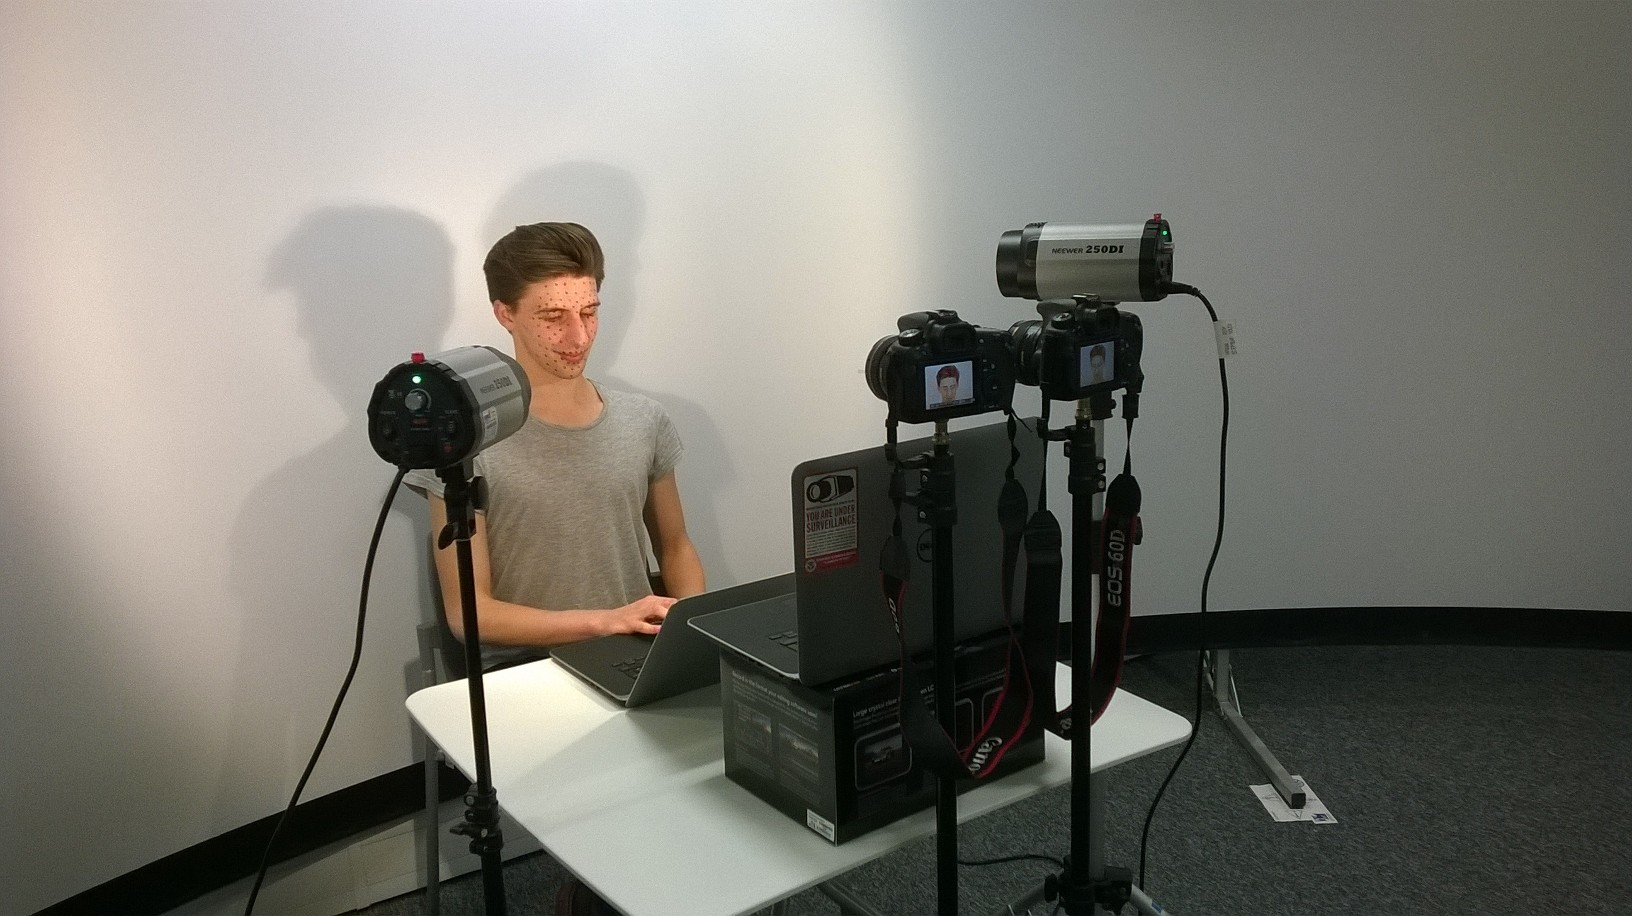
\includegraphics[width=0.7\textwidth]{img/setup1}
\caption{\tiny{The data capture session using two DSLR cameras in stereo.}}
\end{figure}
\end{center}

\end{frame}



\begin{frame}{Face Markers}

\begin{itemize}
\setlength\itemsep{0.5em}
\item Markers are drawn onto the actor's face to track the facial performance.
\end{itemize}

\begin{center}
\begin{figure}
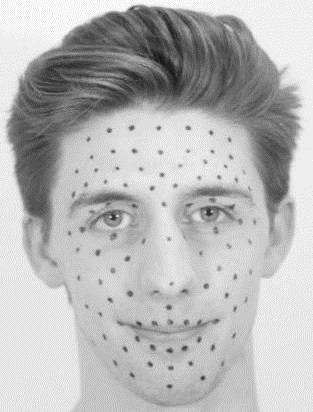
\includegraphics[width=0.35\textwidth]{img/facemarkers} ~
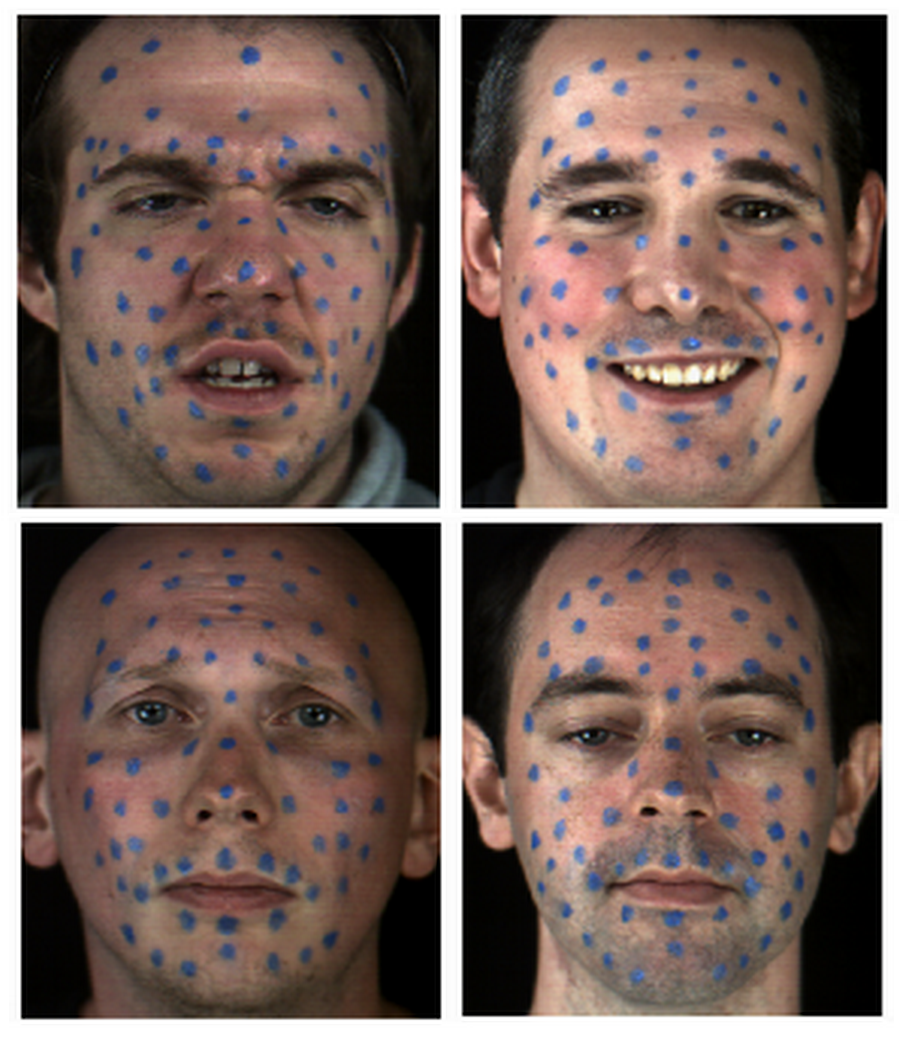
\includegraphics[width=0.4\textwidth]{img/surreydata}
\caption{\tiny{Marker positions were roughly based on the Surrey Audio-Visual Expressed Emotion (SAVEE) Database.}}
\end{figure}
\end{center}

\end{frame}



\begin{frame}{Stereo Calibration}

\begin{itemize}
\setlength\itemsep{0.5em}
\item A checkerboard pattern used to calibrate stereo camera setup.
\item Obtain the cameras' intrinsic and external parameters.
\item Compute the projection matrices and fundamental matrix.
\end{itemize}

\begin{center}
\begin{figure}
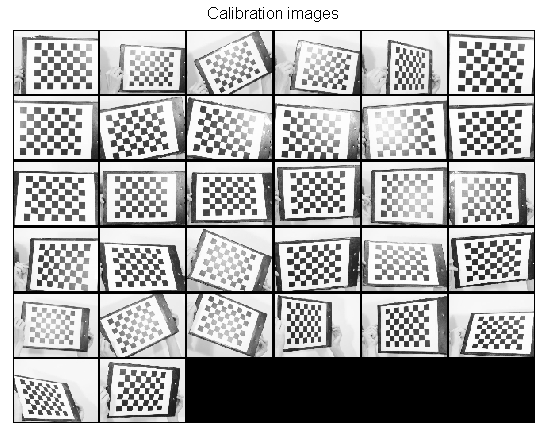
\includegraphics[width=0.4\textwidth]{img/checkerboard} ~
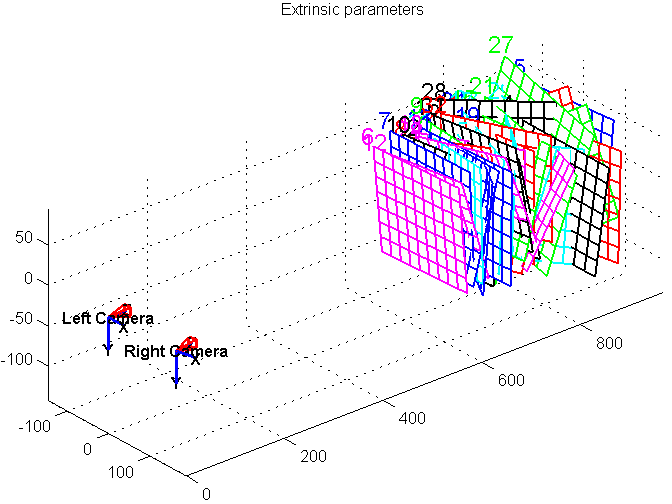
\includegraphics[width=0.42\textwidth]{img/calib}
\caption{\tiny{The stereo cameras were calibrated using a checkerboard pattern.}}
\end{figure}
\end{center}

\end{frame}



\begin{frame}{Stereo Rectification}

\begin{itemize}
\setlength\itemsep{0.5em}
\item Using the camera parameters we rectify each stereo pair for a captured image sequence.
\item Corresponding epipolar lines lie on the same pixel rows.
\item Reduces correspondence problem to a 1D search.
\end{itemize}

\begin{center}
\begin{figure}
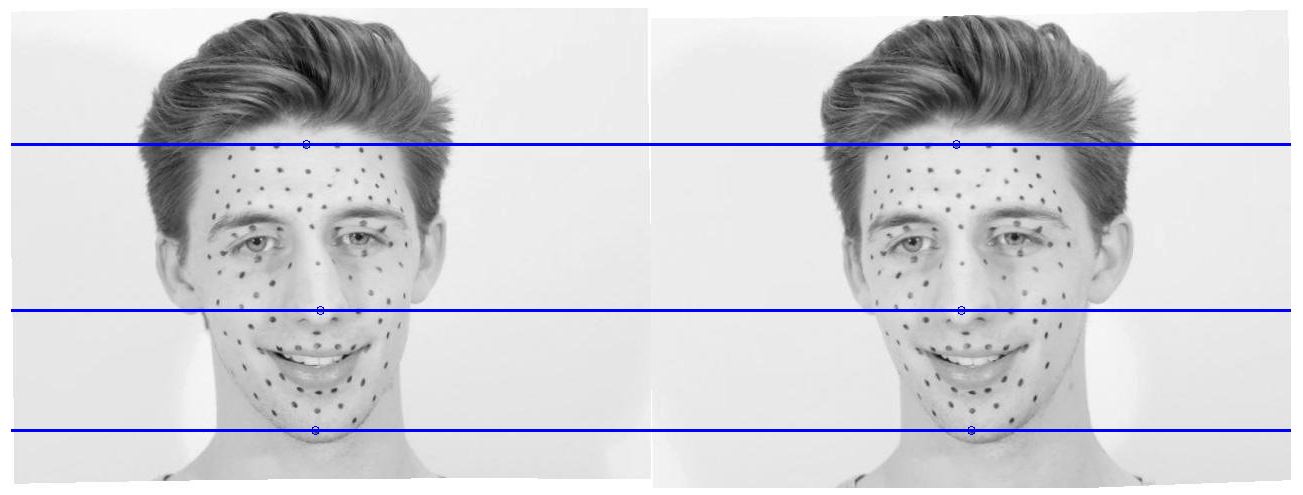
\includegraphics[width=0.8\textwidth]{img/epipolarlines}
\caption{\tiny{Each frame of an image sequence is stereo rectified.}}
\end{figure}
\end{center}

\end{frame}



\begin{frame}{Initial Marker Detection}

\begin{itemize}
\setlength\itemsep{0.5em}
\item Face markers are detected by computing SIFT features in the left image of the first frame.
\item Wrongly detected pixels can be removed and additional points included interactively.
\end{itemize}

\begin{center}
\begin{figure}
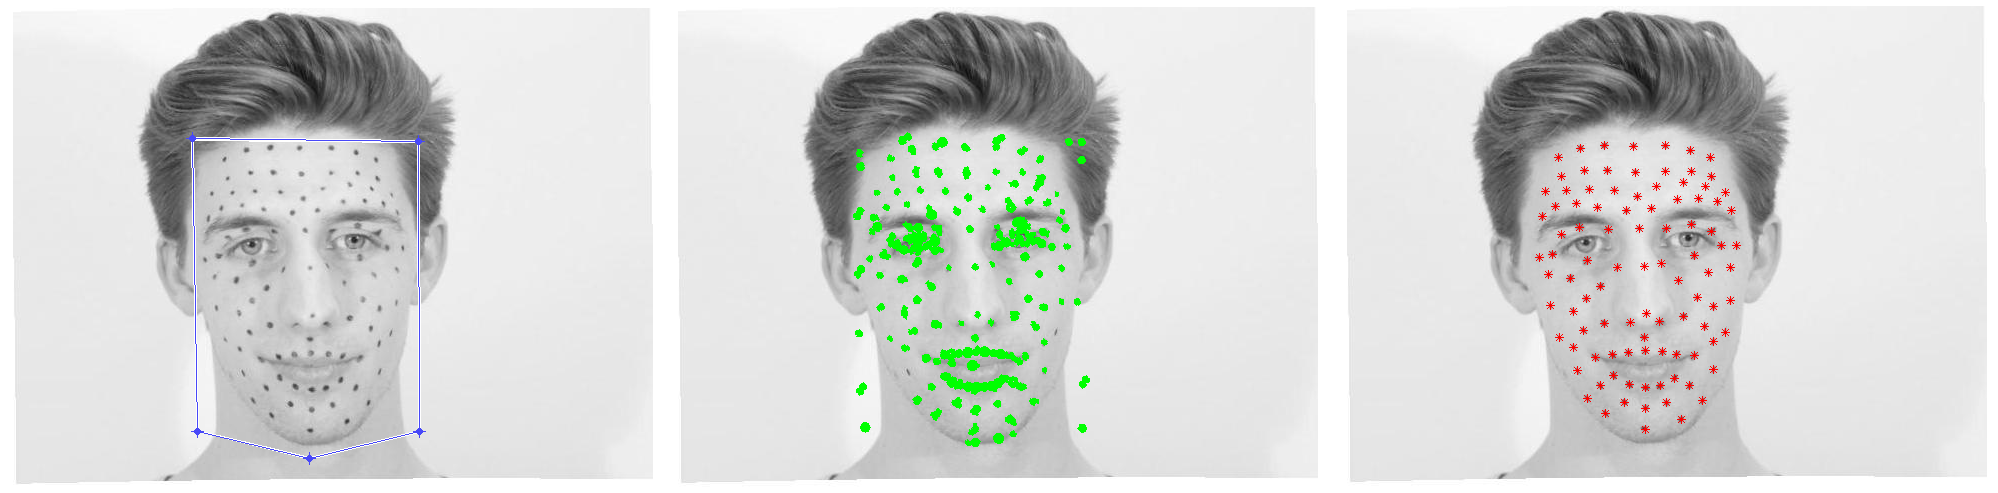
\includegraphics[width=1.0\textwidth]{img/detection}
\caption{\tiny{Markers on the face are detected using SIFT features.}}
\end{figure}
\end{center}

\end{frame}



\begin{frame}{Feature Matching}

\begin{itemize}
\setlength\itemsep{0.5em}
\item Corresponding markers in the right image are found by searching along the corresponding epipolar lines.
\item Matching features are found by computing the normalised cross-correlation for image patches around each feature point.
\end{itemize}

\begin{center}
\begin{figure}
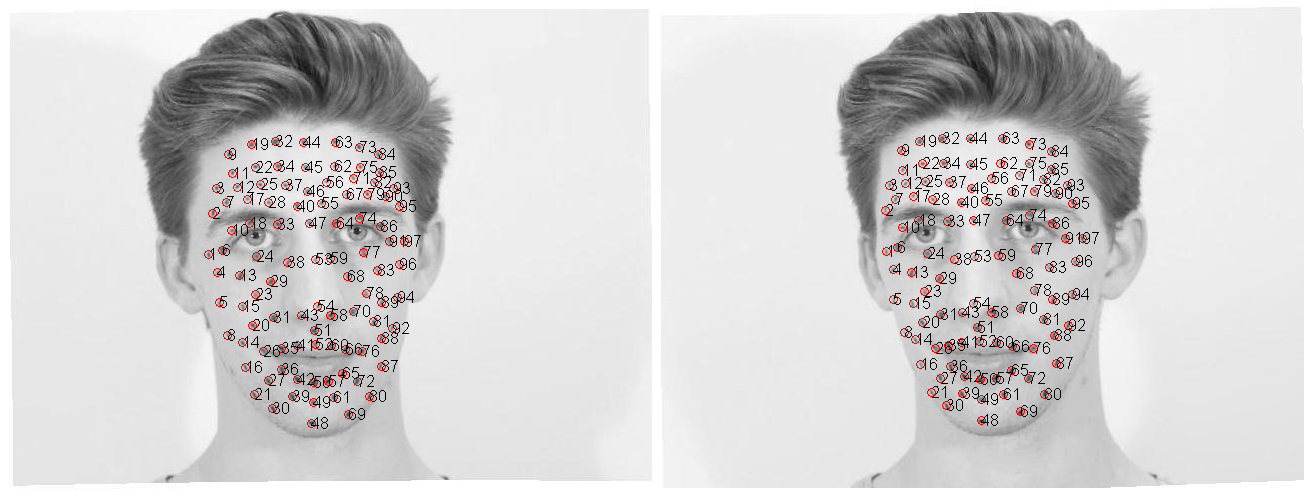
\includegraphics[width=1.0\textwidth]{img/matching}
\caption{\tiny{Corresponding markers are found in the right image.}}
\end{figure}
\end{center}

\end{frame}



\begin{frame}{Marker Tracking}

\begin{itemize}
\setlength\itemsep{0.5em}
\item We track the face markers throughout the entire image sequence using the KLT tracking algorithm.
\end{itemize}

\begin{center}
\begin{figure}
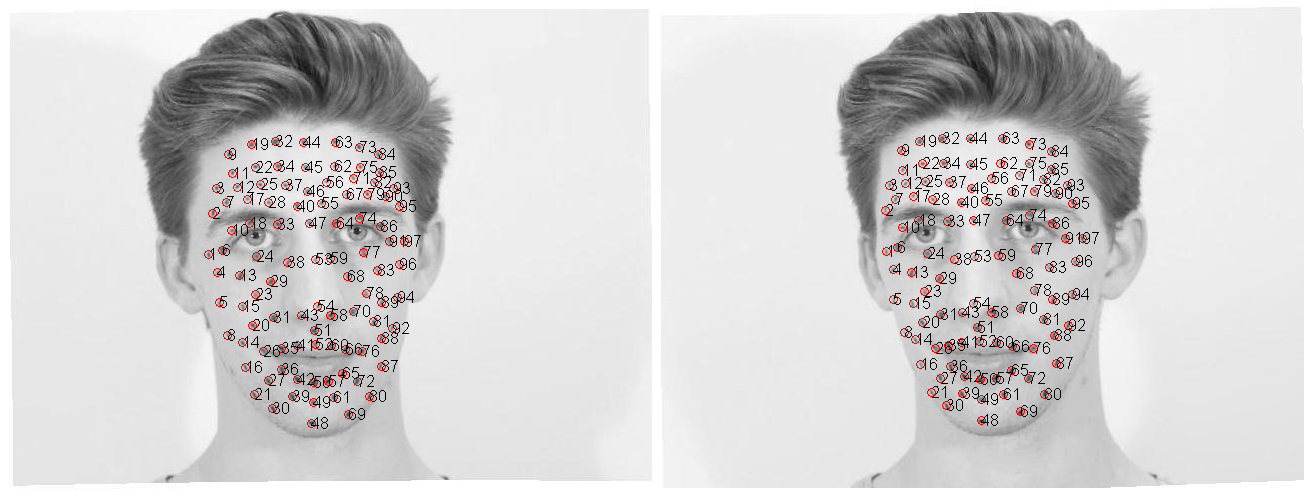
\includegraphics[width=1.0\textwidth]{img/matching}
\caption{\tiny{Corresponding markers are found in the right image.}}
\end{figure}
\end{center}

\end{frame}



\begin{frame}{Sparse Reconstruction}

\begin{itemize}
\setlength\itemsep{0.5em}
\item Using the known camera projection matrices, we compute a sparse 3D reconstruction for every frame.
\end{itemize}

\begin{center}
\begin{figure}
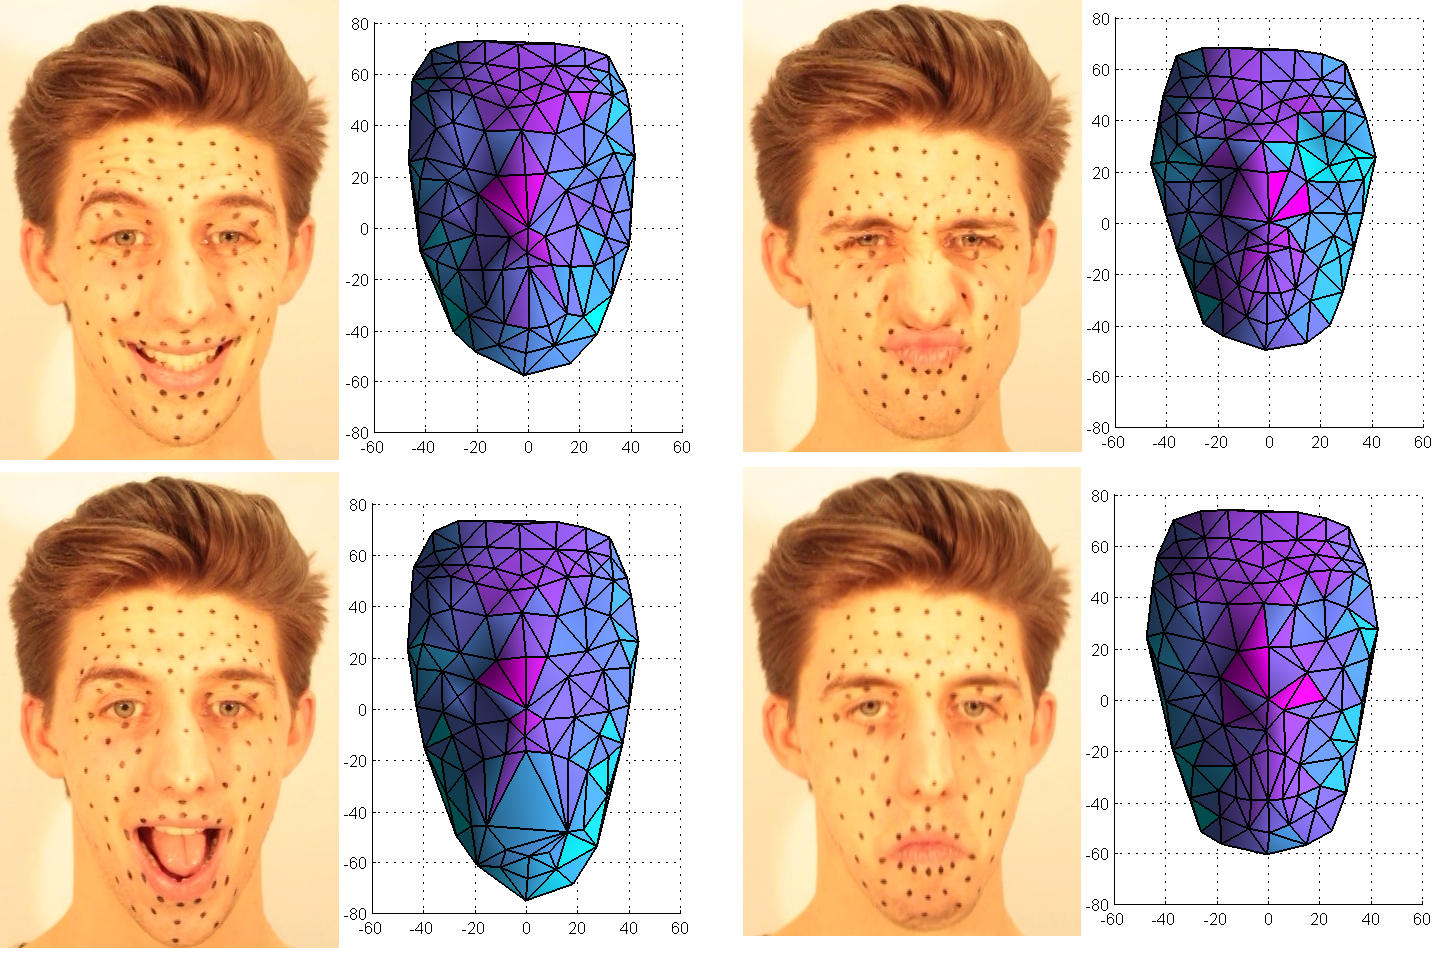
\includegraphics[width=0.8\textwidth]{img/faces}
\caption{\tiny{A sample of reconstructed frames from a captured image sequence.}}
\end{figure}
\end{center}

\end{frame}



\begin{frame}{Head Stabilisation}

\begin{itemize}
\setlength\itemsep{0.5em}
\item We attempt to remove the rigid head motion by performing Procrustes alignment.
\item The head pose in each frame of an image sequence is aligned to the neutral pose. 
\item The 3D point trajectories are also smoothed to remove jittery head motion. 
\end{itemize}

\begin{center}
\begin{figure}
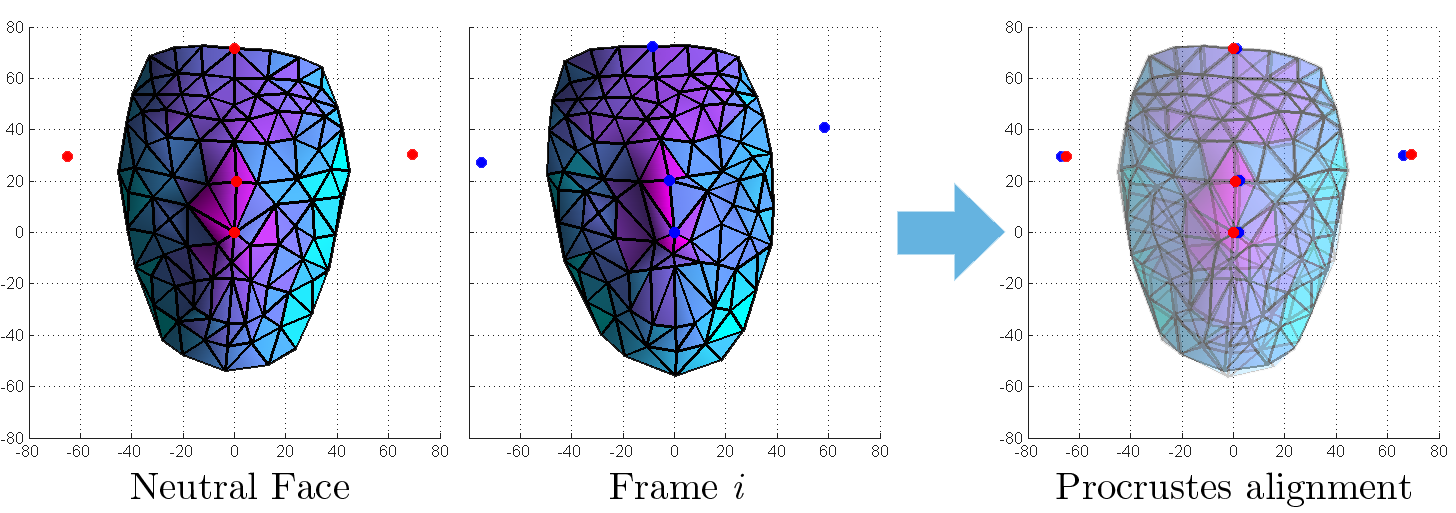
\includegraphics[width=0.8\textwidth]{img/procrustes}
\caption{\tiny{Rigid head motion is removed using Procrustes analysis.}}
\end{figure}
\end{center}

\end{frame}

%----------------------------------------------------------------------
\section{Ieva's Part}
\begin{frame}{Frame name}

\end{frame}


\begin{frame}{Frame name}

\end{frame}


%----------------------------------------------------------------------
\section{Garoe's Part}
\begin{frame}{Frame name}

\end{frame}


\begin{frame}{Frame name}

\end{frame}


%----------------------------------------------------------------------
\section{Results}
\begin{frame}{Frame name}
%\begin{center}
%\begin{figure}
%\movie[width=0.45\textwidth, autostart, loop]
%        {\includegraphics[width=0.25\textwidth]{img/arkanoid}}{img/arkanoid1.mov}
%~
%%,showcontrols
%\caption*{\tiny{Left shows rigid body physics, right shows crossplatform interaction.}}
%\end{figure}
%\end{center}
\end{frame}


\begin{frame}{Frame name}

\end{frame}



%\begin{center}
%\begin{figure}
%\includegraphics[width=0.5\textwidth]{img/6phongReflexion} ~
%\includegraphics[width=0.5\textwidth]{img/8phongShading}
%\caption*{\tiny{Left shows flat shading, right shows Gouraud shading.}}
%\end{figure}
%\end{center}
%
%\begin{itemize}
%\setlength\itemsep{0.5em}
%\item 
%\end{itemize}

%\begin{multicols}{2}
%\begin{figure}[b!]
%\includegraphics[width=0.4\textwidth]{img/cloth_directions}
%\end{figure}
%
%\vfill
%\columnbreak
%\vspace*{\fill}
%\small{where $F$ are Fresnel terms, $\eta$ are Fresnel coefficients, $g$ is a Gaussian lobe, $k_d$ is a scattering constant, $\gamma$ are Gaussian widths, $\theta_h = (\theta_i+\theta_r)/2$ and $\phi_d = \phi_i-\phi_r$. }
%\end{multicols}


%----------------------------------------------------------------------

\end{document}
